\documentclass{article}
\usepackage{hyperref}
\usepackage{listings}

\usepackage{Sweave}
\begin{document}
\input{report-concordance}


\section{Understanding the problem}

Tasks to accomplish

Obtaining the data - Can you download the data and load/manipulate it in R?

Familiarizing yourself with NLP and text mining - Learn about the basics of natural language processing and how it relates to the data science process you have learned in the Data Science Specialization.

\subsection{Obtaining the data}

Download the data from Amazon S3.

Reference to the website which is the original source of the corpus, maintained by \href{http://www.corpora.heliohost.org}{Hans Christensen}

The dataset contains news, blogs and tweets in four different languages, English, German, Russian and Finish.


References:
Corpus website
Dataset description. Lines, sizes, etc.
tm and tau libraries
Corpus statistics



Questions to consider

What do the data look like?

Summary statistics about the data sets.

basic summaries of the three files? Word counts, line counts and basic data tables

The english Corpus has three datasets, with the following statistics:

Twitter: Small sentence(s), maximum number of characters observed is 213. There are 167 million characters, in 30 million words, in 2.3 million tweets.
Blogs: Paragraphs. Multiple sentences per blog. Largest sentence has 40835 characters. In total, this dataset has 37 million words in less than a million lines.
News: Paragraphs. Multiple sentences. Largest sentence has 11384 characters, total words are 30 million in 1 million lines.

\begin{lstlisting}
> docs<-Corpus(DirSource(file.path(".", "dataset", "en_US")))

\end{lstlisting}

Where do the data come from?

Twitter
Blogs
News

Can you think of any other data sources that might help you in this project?

Mailboxes.
Facebook/googleplus/linkedin.
Twitter stream.


\subsection{NLP and text mining}


Familiarizing yourself with NLP and text mining - Learn about the basics of natural language processing and how it relates to the data science process you have learned in the Data Science Specialization.


What are the common steps in natural language processing?

The NLP pipeline involves the following steps:

\begin{itemize}
  \item EOS detection. Are the 3 datasets are already categorized like this?
  \item Tokenization. In the four languages, tokens are words, splitted by space. In the languages that use pictograms, there is no space to seperate the tokens in sentences.
  \item Profanity filtering. 
  \item Part-of-speech tagging. Tag tokens by nouns, verbs, etc.
  \item Chunking. Grammar based analysis of the tagged tokens, not statistical analysis.
  \item Extraction
\end{itemize}


What are some common issues in the analysis of text data?



What is the relationship between NLP and the concepts you have learned in the Specialization?


\section{Data acquisition and cleaning}

Tokenization - identifying appropriate tokens such as words, punctuation, and numbers. Writing a function that takes a file as input and returns a tokenized version of it.

Profanity filtering - removing profanity and other words you do not want to predict.

Loading the data

The load of the data in R has been done in the Corpus data structure, provided by the text mining framework library, tm. That loads the corpus in to the memory.

Data frame is not a good data type to load the text, because it is prone to dimentionality problems. Corpus is using lists.

\begin{lstlisting}
docs<-Corpus(DirSource(file.path(".", "dataset", "en_US")))
\end{lstlisting}

We can address to one of the documents of the Corpus using the document index, and to check one sentence of one document we can continue using nested references.

\begin{lstlisting}
> length(docs[[3]])
[1] 2360148
> docs[[3]][9]
[1] "The new sundrop commercial ...hehe love at first sight"
\end{lstlisting}


Cleaning

non-UTF-8 characters in the corpus

Cleaning by changing all text to lowercase, remove all numbers and punctuation. 

\begin{lstlisting}
sdocs <- tm_map(sdocs, content_transformer(tolower))
sdocs <- tm_map(sdocs, removeNumbers)
sdocs <- tm_map(sdocs, removePunctuation)
sdocs <- tm_map(sdocs, stripWhitespace)
\end{lstlisting}

Removal of english stop-words is not recommended because we are looking for a predictive model for text.

remove smileys and other utf-8 characters



Sampling

Instead of importing the whole files in our dataset via the Corpus(), we can take a sample of the data by manually reading a portion of one file and append it in a sample corpus 

\begin{lstlisting}
con <- file("./dataset/en_US/en_US.blogs.txt", "r")
sampleb <-readLines(con, 1000)
close(con)
con <- file("./dataset/en_US/en_US.news.txt", "r")
samplen <-readLines(con, 1000)
close(con)
con <- file("./dataset/en_US/en_US.twitter.txt", "r")
samplet <-readLines(con, 1000)
close(con)
bdocs <- Corpus(VectorSource(sampleb))
ndocs <- Corpus(VectorSource(samplen))
tdocs <- Corpus(VectorSource(samplet))
\end{lstlisting}

Sentence Tokenization

\begin{lstlisting}
install.packages('qdap')
library(qdap)
sent_detect( "Here is a sentence.  And another one! Where does it end? Nobody knows." )

tm_map(crps , sent_detect, endmarks = c("?", ".", "!", "|", ":", "\n","\r\n"))
corpus <- tm_map(us_files, function(x) strsplit(x, "\\."))

\end{lstlisting}


\subsection{Tokenization}

identifying appropriate tokens such as words, punctuation, and numbers. Writing a function that takes a file as input and returns a tokenized version of it.

Two functions of \textbf{tm} library provide tokenization for R.

\begin{itemize}
\item scan\_tokenizer()
\item MC\_tokenizer()
\item NGramTokenizer()
\end{itemize}

\textbf{scan\_tokenizer()} splits the text of the corpus to a character vector, by using the blankspace as the delimiter. Anything between spaces is considered a word.

\textbf{MC\_tokenizer()} splits the text of the corpus to a character vector, and ignores the punctuation, parenthesis, numbers, etc.

\textbf{NGramTokenizer()} splits a string to n-grams.

\begin{lstlisting}
library('RWeka')
ngram <- 2
options(mc.cores=1)
BigramTokenizer <- function(x) NGramTokenizer(x,Weka_control(min=ngram,max=ngram))
tdm <- TermDocumentMatrix(sdocs, control = list(tokenize = BigramTokenizer))
\end{lstlisting}

\subsection{Profanity filtering}

Profanity filtering - removing profanity and other words you do not want to predict.

Google list of swearing words is available through the dwyl.com website. @jamiew created a list of the words in \href{https://gist.github.com/jamiew/1112488}{his gist}.

Removal of the swearing words doesn't make sense, doesn't help us in prediction:

\begin{lstlisting}
> sdocs[[172]]$content
[1] "\342\200\234: yeah, l could be the bigger person, or you could just shut the fuck up.\342\200\235"
> sdocs <- tm\_map(sdocs, removeWords, swears)
> sdocs[[172]]$content
[1] "\342\200\234: yeah, l could be the bigger person, or you could just shut the  up.\342\200\235"
\end{lstlisting}

Instead, we can remove the whole sentences that have eroneous content:

\begin{lstlisting}
sdocs<-sdocs[-grep(paste(swears,collapse=" | "),sdocs$content)]
\end{lstlisting}


\section{Exploratory analysis}

Tasks to accomplish

Exploratory analysis - perform a thorough exploratory analysis of the data, understanding the distribution of words and relationship between the words in the corpora.

distribution of the words

relationship between the words
 
Understand frequencies of words and word pairs - build figures and tables to understand variation in the frequencies of words and word pairs in the data.

frequencies of the words

frequencies of the word pairs

\subsubsection{Distributions of word frequencies}

Some words are more frequent than others - what are the distributions of word frequencies? 

The distribution is following the Zipf's Law, according to which the frequency of any word is inversely proportional to its rank in the frequency table.

\begin{lstlisting}
par(mfrow=c(4,3))
for (lang in c('en_US','de_DE','fi_FI','ru_RU'))
{
        for (media in c('blogs','news','twitter'))
        {
                con <- file(paste("./dataset/",lang,"/",lang,".",media,".txt",sep=''), "r")
                sample <-readLines(con, 2000)
                close(con)
                sdocs <- VCorpus(VectorSource(sample),  readerControl = list(language=lang))
                dtm <- DocumentTermMatrix(sdocs)
                Zipf_plot(dtm)
                mtext(paste(lang,media))
        }
        
}
title("Word frequency distribution per corpus language and media type, following Zipf's Law", outer=TRUE)
\end{lstlisting}

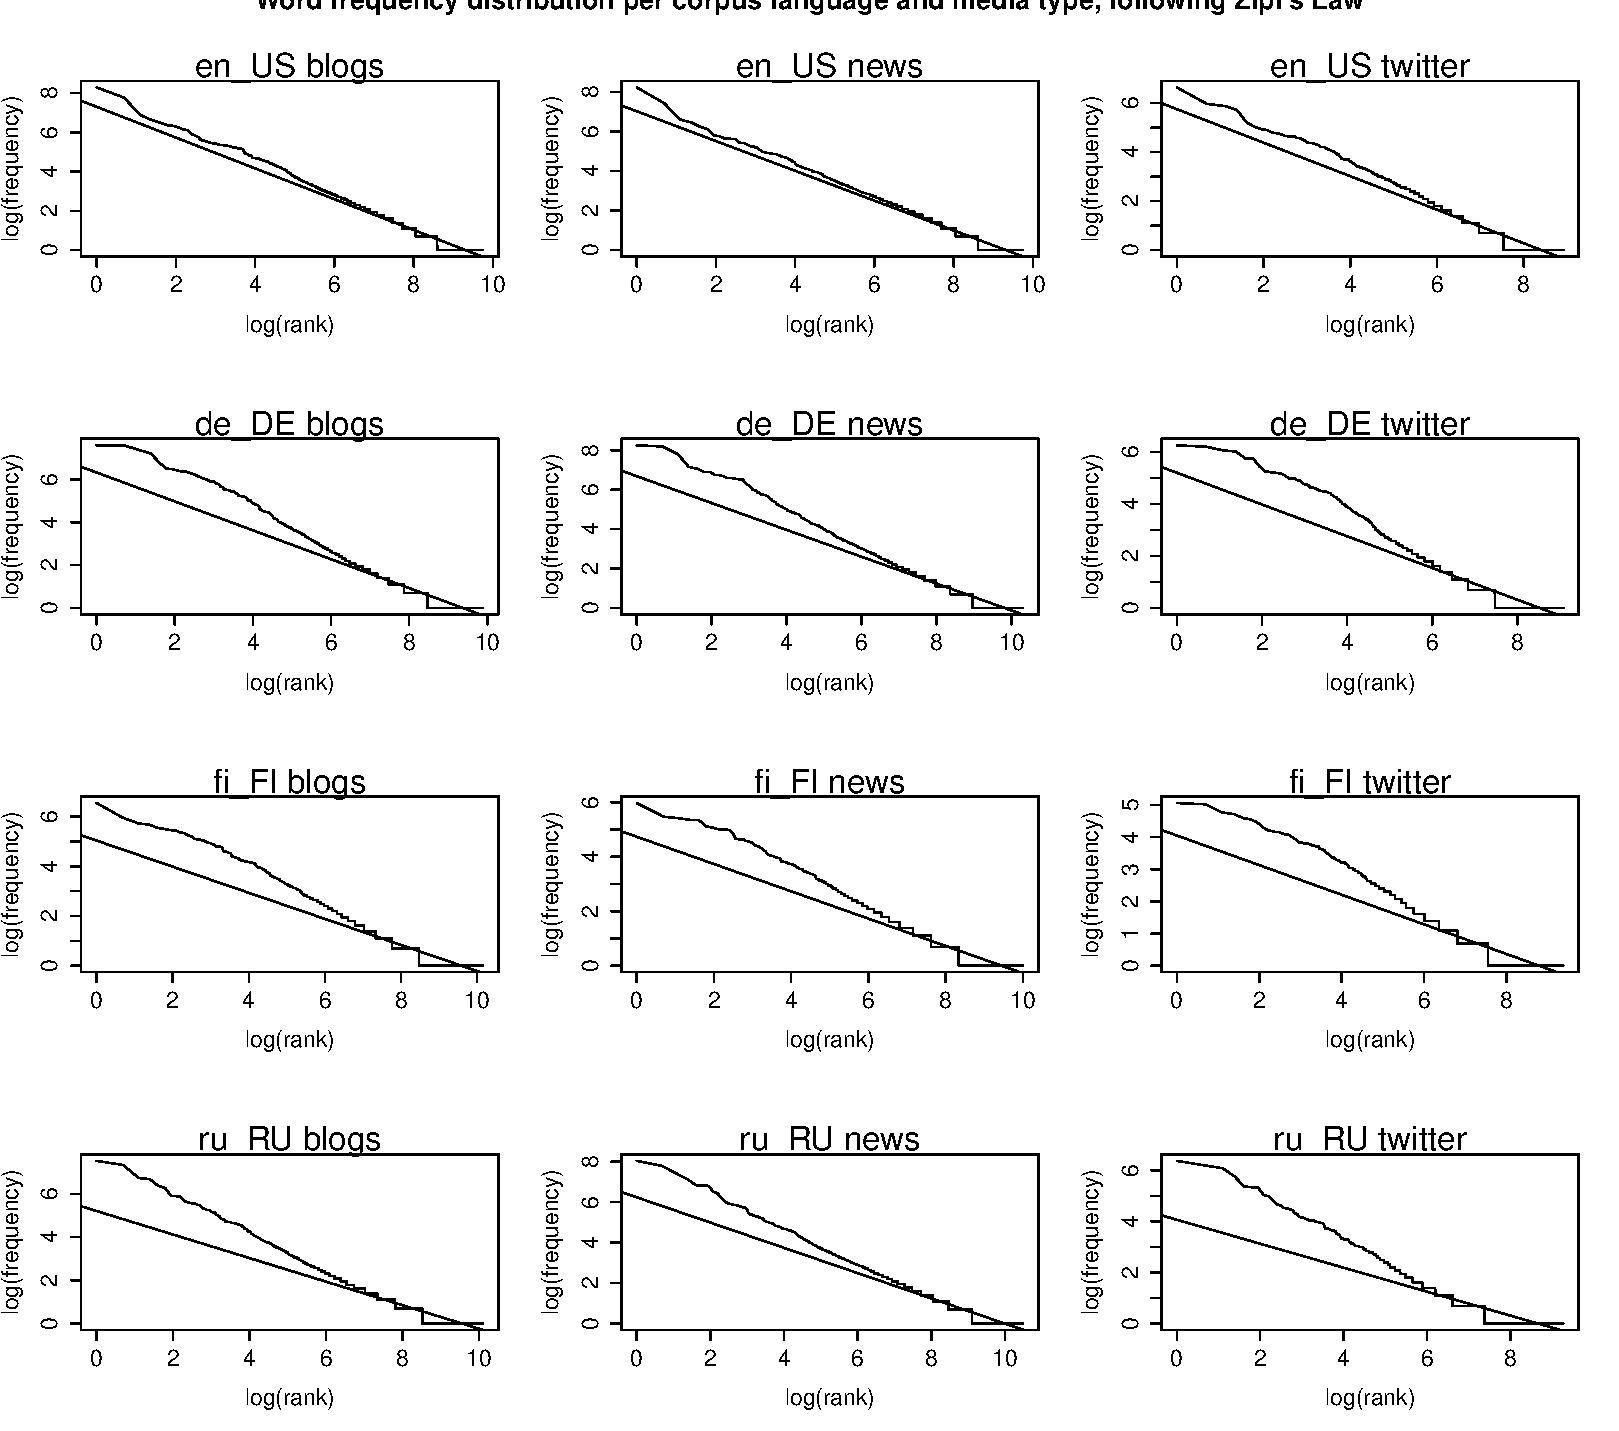
\includegraphics[width=0.98\textwidth]{graphics/zipf.pdf}

What are the frequencies of 2-grams and 3-grams in the dataset? 


\begin{lstlisting}
par(mfrow=c(4,3))
for (lang in c('en_US','de_DE','fi_FI','ru_RU'))
{
        for (media in c('blogs','news','twitter'))
        {
                con <- file(paste("./dataset/",lang,"/",lang,".",media,".txt",sep=''), "r")
                sample <-readLines(con, 2000)
                close(con)
                sdocs <- VCorpus(VectorSource(sample),  readerControl = list(language=lang))
                ngram <- 2
                options(mc.cores=1)
                BigramTokenizer <- function(x) NGramTokenizer(x,Weka_control(min=ngram,max=ngram))
                btdm <- TermDocumentMatrix(sdocs, control = list(tokenize = BigramTokenizer))
                Zipf_plot(btdm)
                mtext(paste(lang,media))
        }
}
title("Bigram frequency distribution per corpus language and media type.", outer=TRUE)
\end{lstlisting}

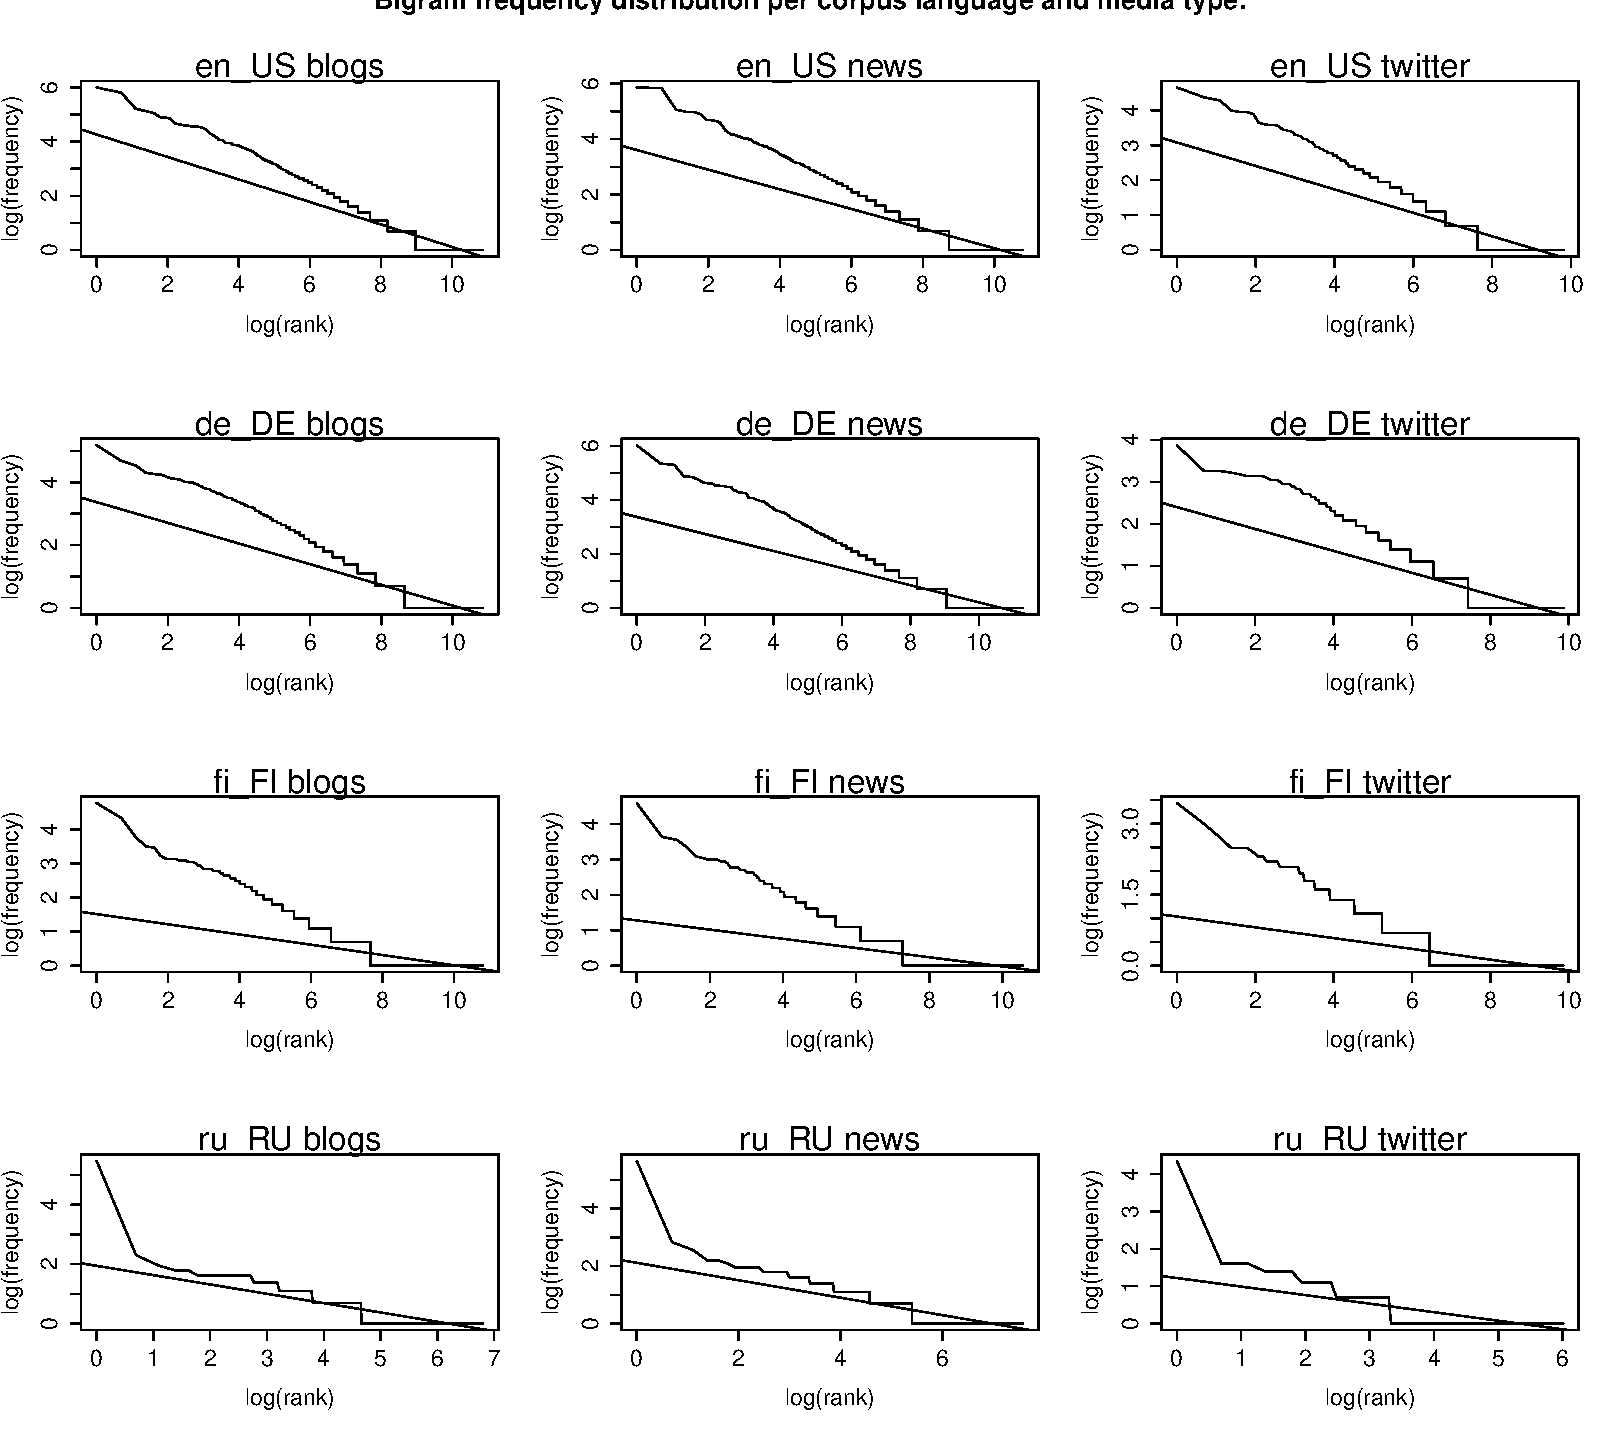
\includegraphics[width=0.98\textwidth]{graphics/bigrams_frequency.pdf}

\begin{lstlisting}
par(mfrow=c(4,3))
for (lang in c('en_US','de_DE','fi_FI','ru_RU'))
{
        for (media in c('blogs','news','twitter'))
        {
                con <- file(paste("./dataset/",lang,"/",lang,".",media,".txt",sep=''), "r")
                sample <-readLines(con, 2000)
                close(con)
                sdocs <- VCorpus(VectorSource(sample),  readerControl = list(language="en_US"))
                ngram <- 3
                options(mc.cores=1)
                TrigramTokenizer <- function(x) NGramTokenizer(x,Weka_control(min=ngram,max=ngram))
                ttdm <- TermDocumentMatrix(sdocs, control = list(tokenize = TrigramTokenizer))
                Zipf_plot(ttdm)
                mtext(paste(lang,media))
        }
}
title("Trigram frequency distribution per corpus language and media type.", outer=TRUE)
\end{lstlisting}

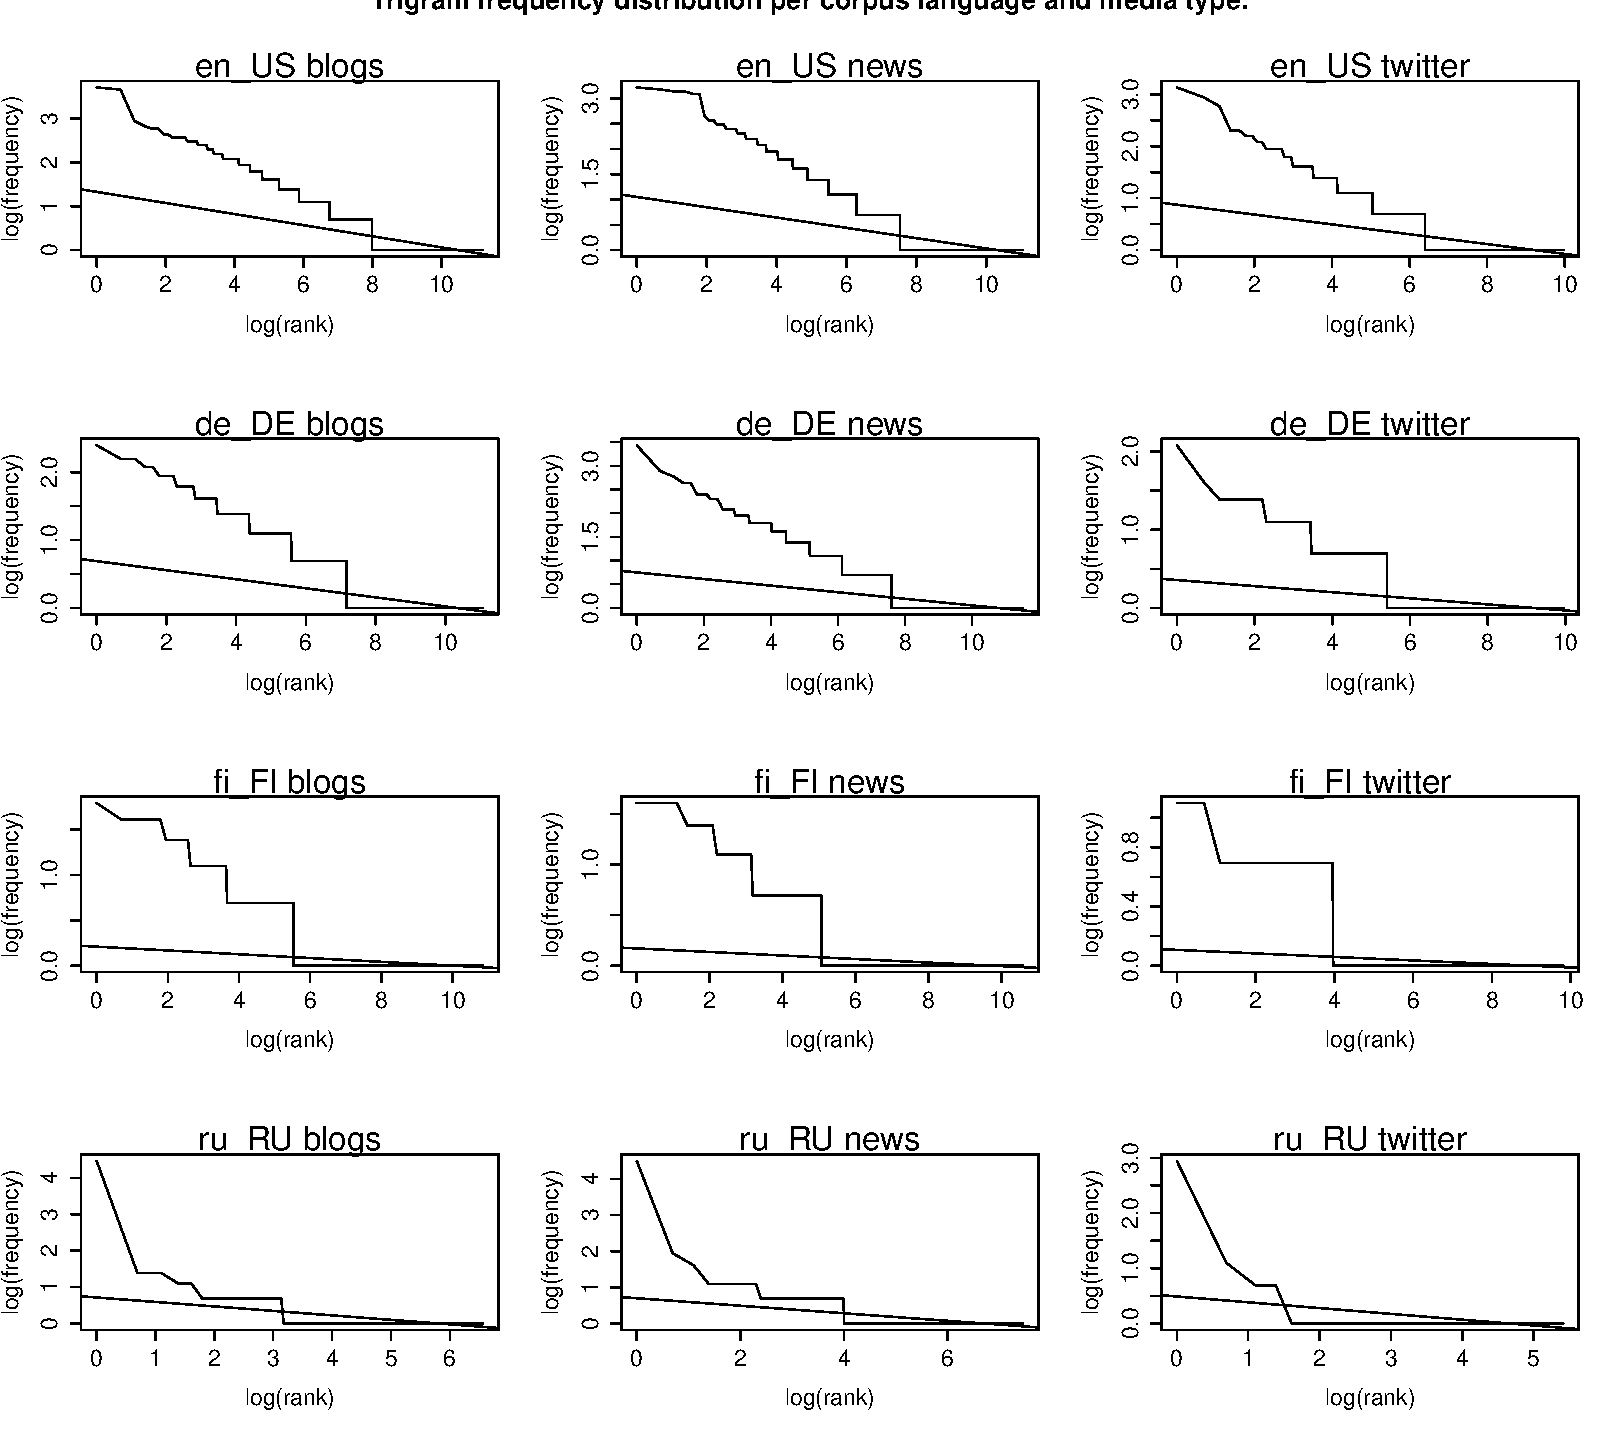
\includegraphics[width=0.98\textwidth]{graphics/trigrams_frequency.pdf}

How many unique words do you need in a frequency sorted dictionary to cover 50% of all word instances in the language? 90%? 

\begin{lstlisting}
dtm <- DocumentTermMatrix(sdocs)
allwords<-length(dtm\$i)
words<-sort(colSums(as.matrix(dtm)),decreasing=TRUE)
perc=.5
suma=0
for(i in 1:allwords)
{
        suma<-suma+words[[i]]
        if(suma>=(perc*allwords))
                {
                print(i)
                break
        }
}
\end{lstlisting}

\begin{center}
    \begin{tabular}{ | l | l | l | l |}
    \hline
    language & twitter & blogs & news \\ \hline
    en\_US &  195  & 116 &  247 \\ \hline
    ru\_RU &  576  & 594 &  711  \\ \hline
    fi\_FI &  1661 & 1665 & 2711  \\ \hline
    de\_DE &  151  & 88 &  143  \\ \hline
    \end{tabular}
\end{center}


How do you evaluate how many of the words come from foreign languages? 

Can you think of a way to increase the coverage -- identifying words that may not be in the corpora or using a smaller number of words in the dictionary to cover the same number of phrases?

\end{document}
